\documentclass{article}

\usepackage{amsmath,amssymb}
\usepackage[ruled,vlined]{algorithm2e}
\usepackage{graphicx}
\graphicspath{ {./images/} }
\usepackage{pgfplotstable}
\usepackage{pgfplots}
\usepackage{float}
\usepackage{hyperref}
\usepackage{framed}

\usepackage{listings}
\usepackage{color}

\definecolor{dkgreen}{rgb}{0,0.6,0}
\definecolor{gray}{rgb}{0.5,0.5,0.5}
\definecolor{mauve}{rgb}{0.58,0,0.82}

\lstset{frame=tb,
  language=C,
  aboveskip=3mm,
  belowskip=3mm,
  showstringspaces=false,
  columns=flexible,
  numbers=left,
  stepnumber=1,
  basicstyle={\small\ttfamily},
  numberstyle=\tiny\color{gray},
  keywordstyle=\color{blue},
  commentstyle=\color{dkgreen},
  stringstyle=\color{mauve},
  breaklines=true,
  breakatwhitespace=true,
  tabsize=3,
  morekeywords={pragma}
}

% Margins
\usepackage[top=2.5cm, left=3cm, right=3cm, bottom=4.0cm]{geometry}
% Colour table cells

% Get larger line spacing in table
\newcommand{\tablespace}{\\[1.25mm]}
\newcommand\Tstrut{\rule{0pt}{2.6ex}}         % = `top' strut
\newcommand\tstrut{\rule{0pt}{2.0ex}}         % = `top' strut
\newcommand\Bstrut{\rule[-0.9ex]{0pt}{0pt}}   % = `bottom' strut

%%%%%%%%%%%%%%%%%
%     Title     %
%%%%%%%%%%%%%%%%%
\title{CS426 Project 3 Report}
\author{Rüzgar Ayan \\ 21801984}
\date{\today}

\begin{document}
\maketitle

\section{Some Assumptions and Notes on Implementation}

\begin{itemize}
    \item The matrix is supposed to be generated with random integers. If the random integers are generated in range [$0$,INT\_MAX], the rank would become equal to $n$ almost every time. So I generated the numbers in range [$0$, $9$].

    \item About checking the dependency of two rows, the project's PDF file says the following:

    \begin{quote}
    "Now we get into the parallel part. If the matrix’s
    dimension is (n,n), for checking the dependency of two rows we have to check all the elements of the rows." 
    \end{quote}
    
    In the following method of my sequential part code, I check all the elements of two rows with the for loop (lines 7-10). Although I could break out of the for loop whenever we go inside the if statement, I didn't do it because PDF was telling to check all the elements.
    
    \begin{lstlisting}
    int checkIndependentRows(int **matrix, int n, int row1, int row2) {
    	int row1First = matrix[row1][0];
    	int row2First = matrix[row2][0];
    
    	int isIndependent = 0;
    
    	for (int i = 0; i < n; i++) {
    		if (matrix[row1][i] * row2First != matrix[row2][i] * row1First)
    			isIndependent = 1;
    	}
    	
    	return isIndependent;
    }
    \end{lstlisting}
    
    I guess checking all the elements was asked because break is not allowed in OpenMP's parallel for loops. But in case that I misunderstood something, I still added two alternative methods checkIndependentRowsAlternative and checkIndependentRowsAlternative2 to the parallel code that can break out of the for loop once the independency of rows is found.
\end{itemize}

\section{Used Parallelization Strategy} 

While checking the independency of two rows, it is possible to divide both rows into parts and check the independency of these new smaller parts. Using that, we can just make the for loop in the previous code snippet into an "omp parallel for". For independency of the whole rows, at least one pair of these smaller parts must be independent. So, only  a single pragma line is added to the sequential code as follows:

\begin{lstlisting}
int checkIndependentRows(int **matrix, int n, int row1, int row2) {
	int row1First = matrix[row1][0];
	int row2First = matrix[row2][0];

	int isIndependent = 0;
	
	#pragma omp parallel for shared(matrix) reduction(||: isIndependent)
	for (int i = 0; i < n; i++) {
		if (matrix[row1][i] * row2First != matrix[row2][i] * row1First){
			isIndependent = 1;
		}
	}
	
	return isIndependent;
}
\end{lstlisting}

Having the \emph{reduction($\vert\vert$: isIndependet)} in the omp pragma lets us combine the results from all the smaller parts. If at least one thread finds an independent element in their parts, then the result becomes 1.

\section{Results}

The number of threads used in the OpenMP parts was $8$ in these experiments. My runtimes were quite long, so I couldn't run with $n=100000$, instead I put the results for $n=20000$. In order to give all results in a single plot, y axis is in logarithmic scale. 

\begin{figure}[!htb]
    \centering
    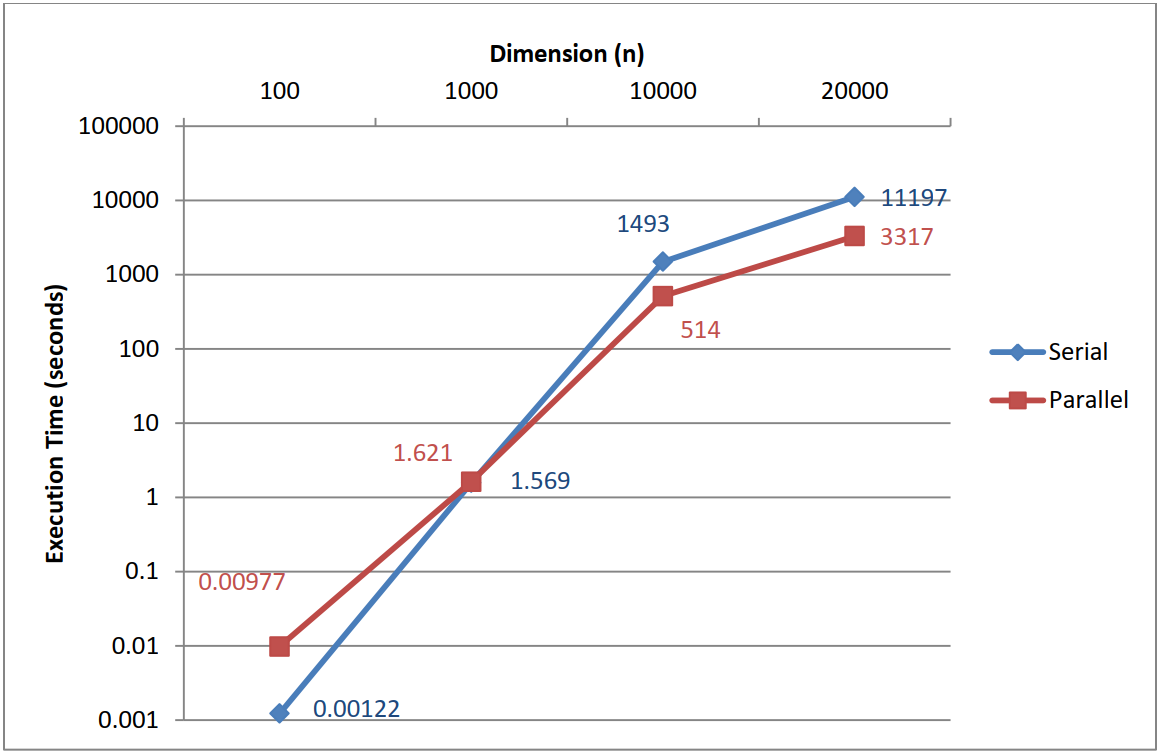
\includegraphics[width=0.75\textwidth]{plot.png}
    \caption{Execution Time Comparison For Serial and Parallel Programs}
\end{figure}

\begin{itemize}
    \item For $n=100$, the parallel program is slower than the serial program. This is expected since we are creating threads just to parallelize a $100$ iteration loop every time we check the dependency of two rows. There is too much overhead.
    \item For $n=1000$, the overheads become smaller in comparison to the total execution time. However, we are still using 8 processors to get the same execution time as with the serial program.
    \item For $n=10000$, parallel program start to perform better than the serial one. The speedup is $2.90$
    \item For $n=20000$, the speedup increases to $3.37$. With this large $n$, I would expect the speedup to be closer to $8$, but parallelization is probably still worth it with these speedups.
\end{itemize}

\section{Other Parts That Could Be Parallelized}

As seen in the previous section, parallel version does not work better than the serial version for small $n$ values. Since we parallelized the innermost part of the algorithm, the overhead of creating threads is a lot. Instead we could parallelize an outer for loop that would let us check the dependency of some row with multiple other rows at the same time. 

One disadvantage is that some load imbalance may occur since the rows that are not independent are eliminated and they are not required to do any more checks. These eliminated rows might be clustered in some regions if there is a pattern in the matrix (not random like in this assignment). We can eliminate this problem by using OpenMP schedule clause with DYNAMIC scheduling. 

As another possibility, we could apply a parallelism to the outermost part so that we have something like thread $1$ checks the dependency of row $1$ with all the other rows while thread $2$ checks the dependency of row $2$ with all the other rows and so on. The currently eliminated rows must be shared between all the threads so that they are not checked again and again unnecessarily. DYNAMIC scheduling can be used for the same purpose again.

\end{document}